\section{Database}\label{sec:testdatabase}
% introduktion
I det følgende vil test og integration af databasen blive beskrevet. Alle komponenter er udviklet iterativt og integreret løbende.

Nogle af billederne som er taget af kørte enhedstest er for store til at kunne være i nedstående afsnit. Disse kan findes i Appendix~\ref{app:figs} på side~\pageref{app:figs}.

\subsection{UserAccess}
% klassens opgave... 
\textit{UserAccess} har til ansvar at håndtere operationer som tager \textit{User}'s ind og up af databasen. Klassen er implementeret som det første i DAL og har dannet grundlag for videre udvikling.

\subsubsection{Testdetaljer}
% beskrivelse af coverage procent og antallet af test, samt begrundelse for begge.
\textit{UserAccess.Unit.Test} har en coverage procent på 100\% (figur~\ref{fig:useraccesscoverage}) og er dækket af 33 test (figur~\ref{fig:useraccessunittest}). Med disse test er både normale brugs- og fejlscenarier dækket.

% BILLEDE AF KØRTE UNITTEST
\begin{figure}[h]
\centering
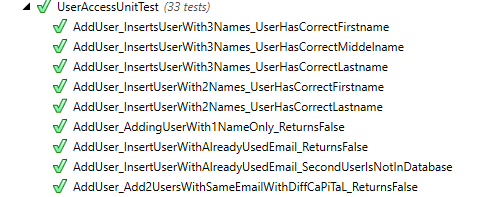
\includegraphics[width=0.9\linewidth]{figs/test/useraccessunittest}
\caption{Unittest for UserAccess.}
\label{fig:useraccessunittest}
\end{figure}

\subsubsection{Testbeskrivelse}
% hvordan div. test er valgt og hvad I specielt var opmærksom på under udviklign af test.
For hver metode er det normale brugsscenarie identificeret og testet for forskellige kombinationer. Herefter problemerne forsøgt identificeret og taget højde for.

% BILLEDE AF COVERAGE KØRT
\begin{figure}[h]
	\centering
	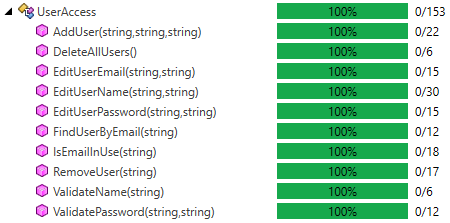
\includegraphics[width=0.7\linewidth]{figs/test/useraccesscoverage}
	\caption{Coverage for UserAccess.}
	\label{fig:useraccesscoverage}
\end{figure} 

% hvad var let/svært at teste etc.

\subsection{PoolAccess}
% klassens opgave... 
\textit{PoolAccess} har til ansvar at håndtere operationer som tager \textit{Pool}'s ind og up af databasen, samt forbinde en indsæt pool til en Bruger. 

\subsubsection{Testdetaljer}
% beskrivelse af coverage procent og antallet af test, samt begrundelse for begge.
\textit{PoolAccess.Unit.Test} har en coverage procent på 100\% (figur~\ref{fig:poolaccesscoverage}) og er dækket af 41 test (figur~\ref{fig:poolaccessunittest}). Med disse test er både normale brugs- og fejlscenarier dækket.

% BILLEDE AF KØRTE UNITTEST
\begin{figure}[h]
	\centering
	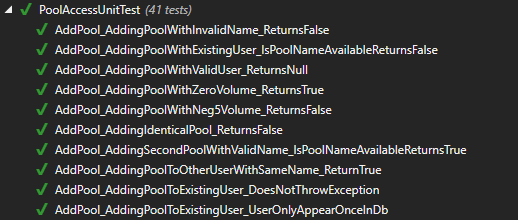
\includegraphics[width=0.8\linewidth]{figs/test/poolaccessunittest}
	\caption{Unittest for PoolAccess.}
	\label{fig:poolaccessunittest}
\end{figure}

\subsubsection{Testbeskrivelse}
% hvordan div. test er valgt og hvad I specielt var opmærksom på under udviklign af test. 
% hvad var let/svært at teste etc.
For hver metode er det normale brugsscenarie identificeret og testet for forskellige kombinationer. Herefter problemerne forsøgt identificeret og taget højde for.\todo{improve pree}

% BILLEDE AF COVERAGE KØRT
\begin{figure}[h]
	\centering
	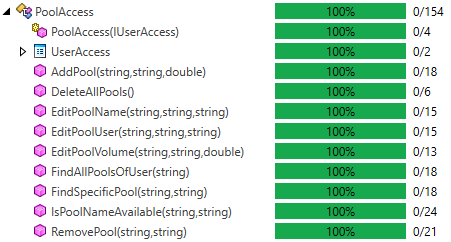
\includegraphics[width=0.7\linewidth]{figs/test/poolaccesscoverage}
	\caption{Coverage for PoolAccess.}
	\label{fig:poolaccesscoverage}
\end{figure}

\subsection{DataAccess}
% klassens opgave... 
\textit{DataAccess} har til ansvar at oprette et dataset for en pool og i den forbindelse registrere tidspunktet for en måling. Yderligere gør klassen det muligt at finde tilbage til den pool som målingerne høre til.

\subsubsection{Testdetaljer}
% beskrivelse af coverage procent og antallet af test, samt begrundelse for begge.
\textit{DataAccess.Unit.Test} har en coverage procent på 100\% (figur~\ref{fig:dataaccesscoverage}) og er dækket af 41 test (figur~\ref{fig:dataaccessunittest}). Med disse test er både normale brugs- og fejlscenarier dækket.

% BILLEDE AF KØRTE UNITTEST
\begin{figure}[h]
	\centering
	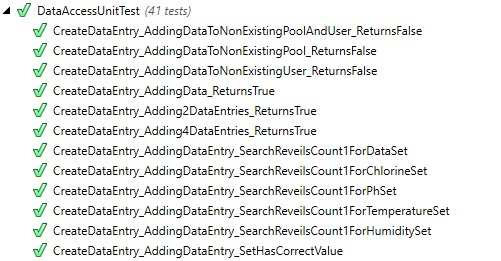
\includegraphics[width=0.9\linewidth]{figs/test/dataaccessunittest}
	\caption{Unittest for DataAccess.}
	\label{fig:dataaccessunittest}
\end{figure}

\subsubsection{Testbeskrivelse}
% hvordan div. test er valgt og hvad I specielt var opmærksom på under udviklign af test. 
% hvad var let/svært at teste etc.
For hver metode er det normale brugsscenarie identificeret og testet for forskellige kombinationer. Herefter problemerne forsøgt identificeret og taget højde for.\todo{improve pree}

% BILLEDE AF COVERAGE KØRT
\begin{figure}[h]
	\centering
	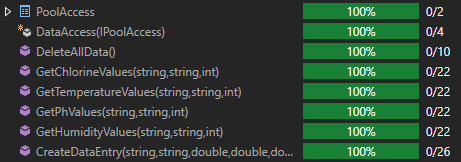
\includegraphics[width=0.7\linewidth]{figs/test/dataaccesscoverage}
	\caption{Coverage for DataAccess.}
	\label{fig:dataaccesscoverage}
\end{figure}